\documentclass[mathserif]{beamer}
\usepackage[utf8]{inputenc}
\usepackage[T1]{fontenc}
\usepackage{array}
\usepackage{amsmath,amssymb,latexsym,epic,eepic,epsfig,graphics,psfrag}
\usepackage{amsfonts,amsbsy}
\usepackage{subfigure}
\definecolor{mygray}{RGB}{244,244,244}
\usepackage[scaled]{beramono}
\usepackage{listings}
\lstset {                 % A rudimentary config that shows off some features.
    language=R,
    basicstyle=\scriptsize\ttfamily, % Without beramono, we'd get cmtt, the teletype font.
    commentstyle=\textit, % cmtt doesn't do italics. It might do slanted text though.
    keywordstyle=,
    identifierstyle=,
    aboveskip=12pt,
    abovecaptionskip=6pt,
    framextopmargin=4pt,
    framexbottommargin=4pt,
    framexleftmargin=4pt,
    framexrightmargin=4pt,
    xleftmargin=4pt,
    xrightmargin=4pt,
    backgroundcolor=\color{mygray},
    frame=single,
    showstringspaces=false,
    captionpos=b,
    tabsize=4            % Or whatever you use in your editor, I suppose.
}
\newcommand\myvec[1]{\boldsymbol{#1}}
\newcommand\myverb[1]{{\footnotesize\texttt{#1}}}
\newcommand\Corr[1]{\textrm{Corr}[#1]}
\newcommand\given{\,|\,}
\newcommand\respath[1]{../results/#1}
\usefonttheme{structurebold}
\usetheme{Copenhagen}
\author{Anders Hørsted -- s082382}
\institute{02433 Hidden Markov Models}
\date{May 31th 2012}


\title[Presentation of exercise 3]{Presentation of written exercise 3}
\begin{document}

\begin{frame}
\titlepage
\end{frame}

\begin{frame}{A few remarks about the report}
    \begin{itemize}
        \item The notation for random variables is inconsistent. When discussing exponential smoothing and ARIMA $y_t$ is used. When discussing Hidden Markov Models $Y_t$ is used.
        \item In the tables with parameter estimates, the indices of the transition probabilities are interchanged. So $\gamma_{ij}$ is really $\gamma_{ji}$ for all $i,j$.
    \end{itemize}
\end{frame}

\begin{frame}{The data}
    \begin{figure}
    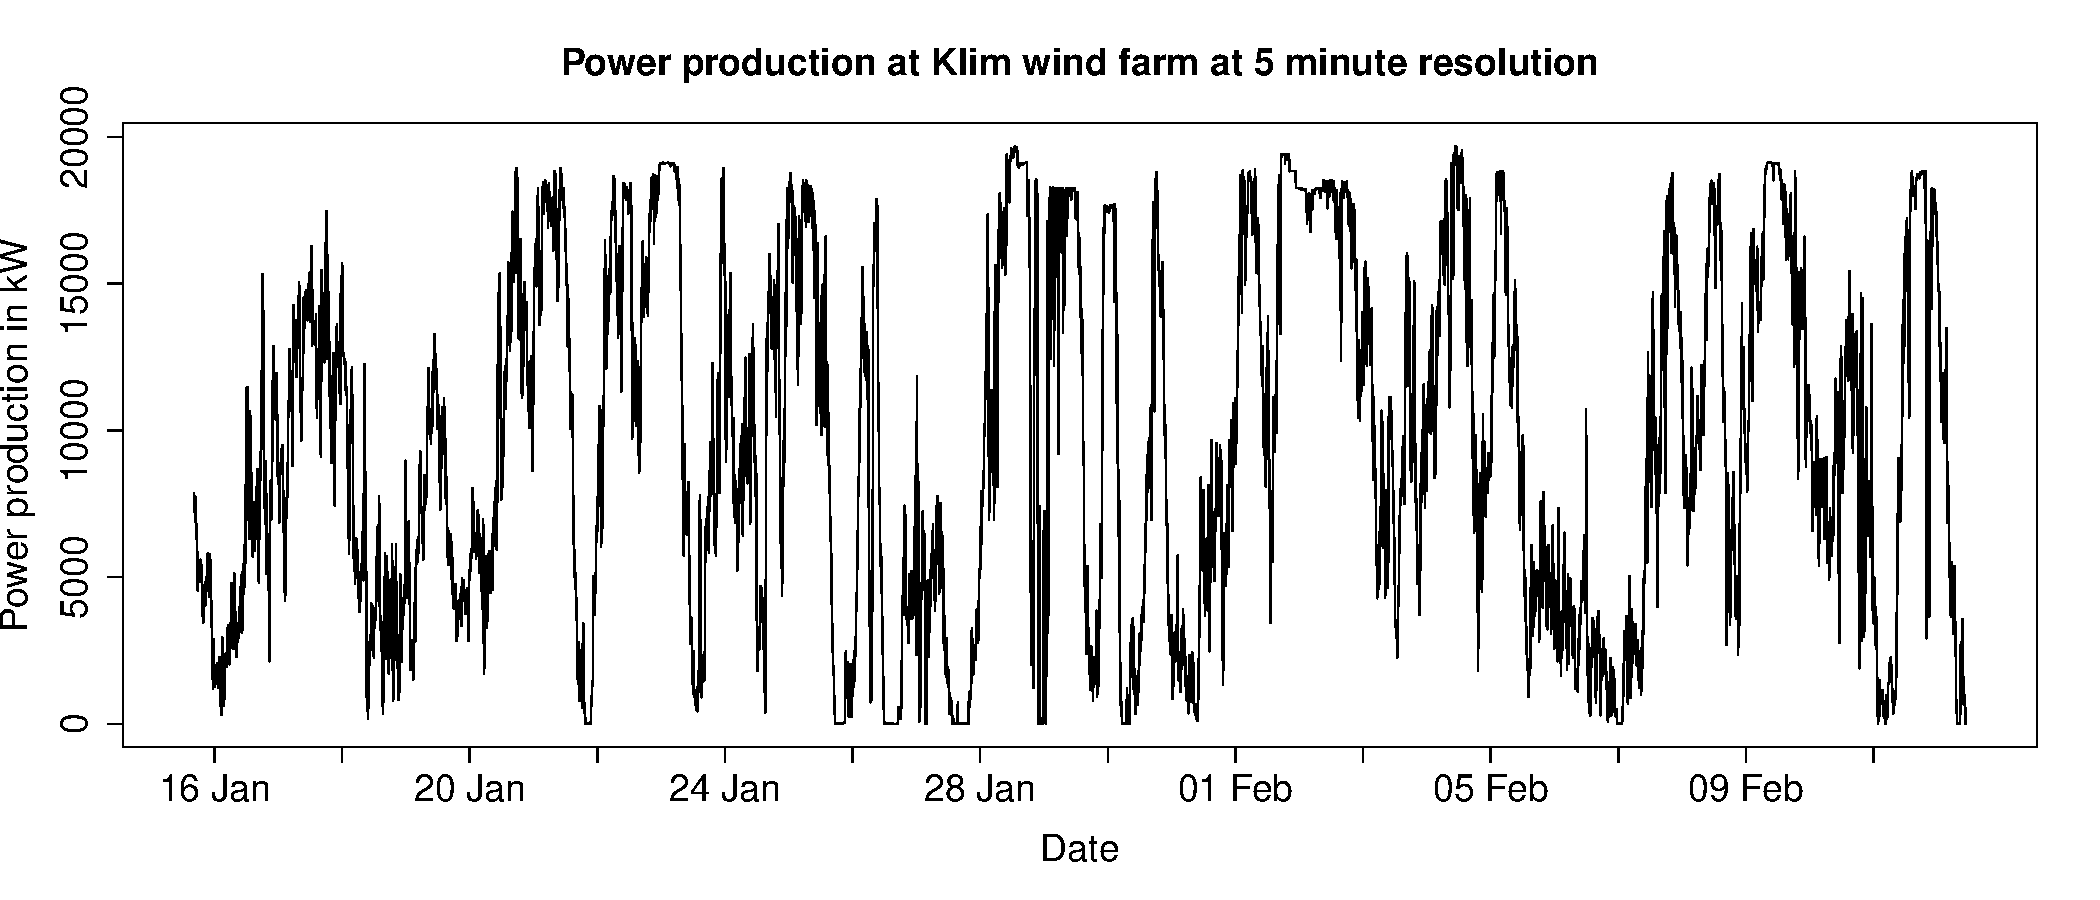
\includegraphics[width=300px]{../plots/training-dataset.pdf}
    \end{figure}
    \begin{itemize}
        \item Measurements of power production at Klim wind farm
        \item Data is bounded on the interval $[0, 21000]$
        \item First 8000 measurements used as training data. 2000 used for performance evaluation.
    \end{itemize}
\end{frame}

\begin{frame}{The task}
    The problem description was open ended. In short form the task was to analyse the data, using various methods for time series analysis.
\end{frame}

\begin{frame}{Exponential smoothing}
    Using the framework presented in (Hyndman08\footnote{{\it Forecasting with Exponential Smoothing - The State Space Approach}, Rob Hyndman et. al.}), a simple exponential smoothing was found to best forecast the data. The smoothing constant was found as $\alpha=0.9999\approx 1$, which gives the model
    \begin{equation*}
        Y_t = Y_{t-1} + e_t
    \end{equation*}
    which is just a random walk. The one-step prediction is $\widehat{Y}_{t|t-1}=Y_{t-1}$ and based on that, the RMSE of the forecasts on the testset was
    \begin{equation*}
        R_{\textrm{RandomWalk}} = 921.33
    \end{equation*}
\end{frame}

\begin{frame}{ARIMA}
    Using the ACF and PACF estimates the best ARIMA model was found to be an ARIMA(1,1,2) model. Estimating the parameters gave the model
    \begin{equation*}
        \nabla Y_t = 0.80\nabla Y_{t-1} - 0.61 e_{t-1} - 0.21 e_{t-2} + e_t
    \end{equation*}
    One step predictions were calculated and the RMSE was found to be
    \begin{equation*}
        R_{\textrm{ARIMA(1,1,2)}} = 874.73
    \end{equation*}
    A large improvement compared with the exponential smoothing forecasts.
\end{frame}

\begin{frame}{ARIMA model check}
    To make an emperical check of the found ARIMA model, a few datasets were simulated from the found model.
    \begin{figure}
    \only<1>{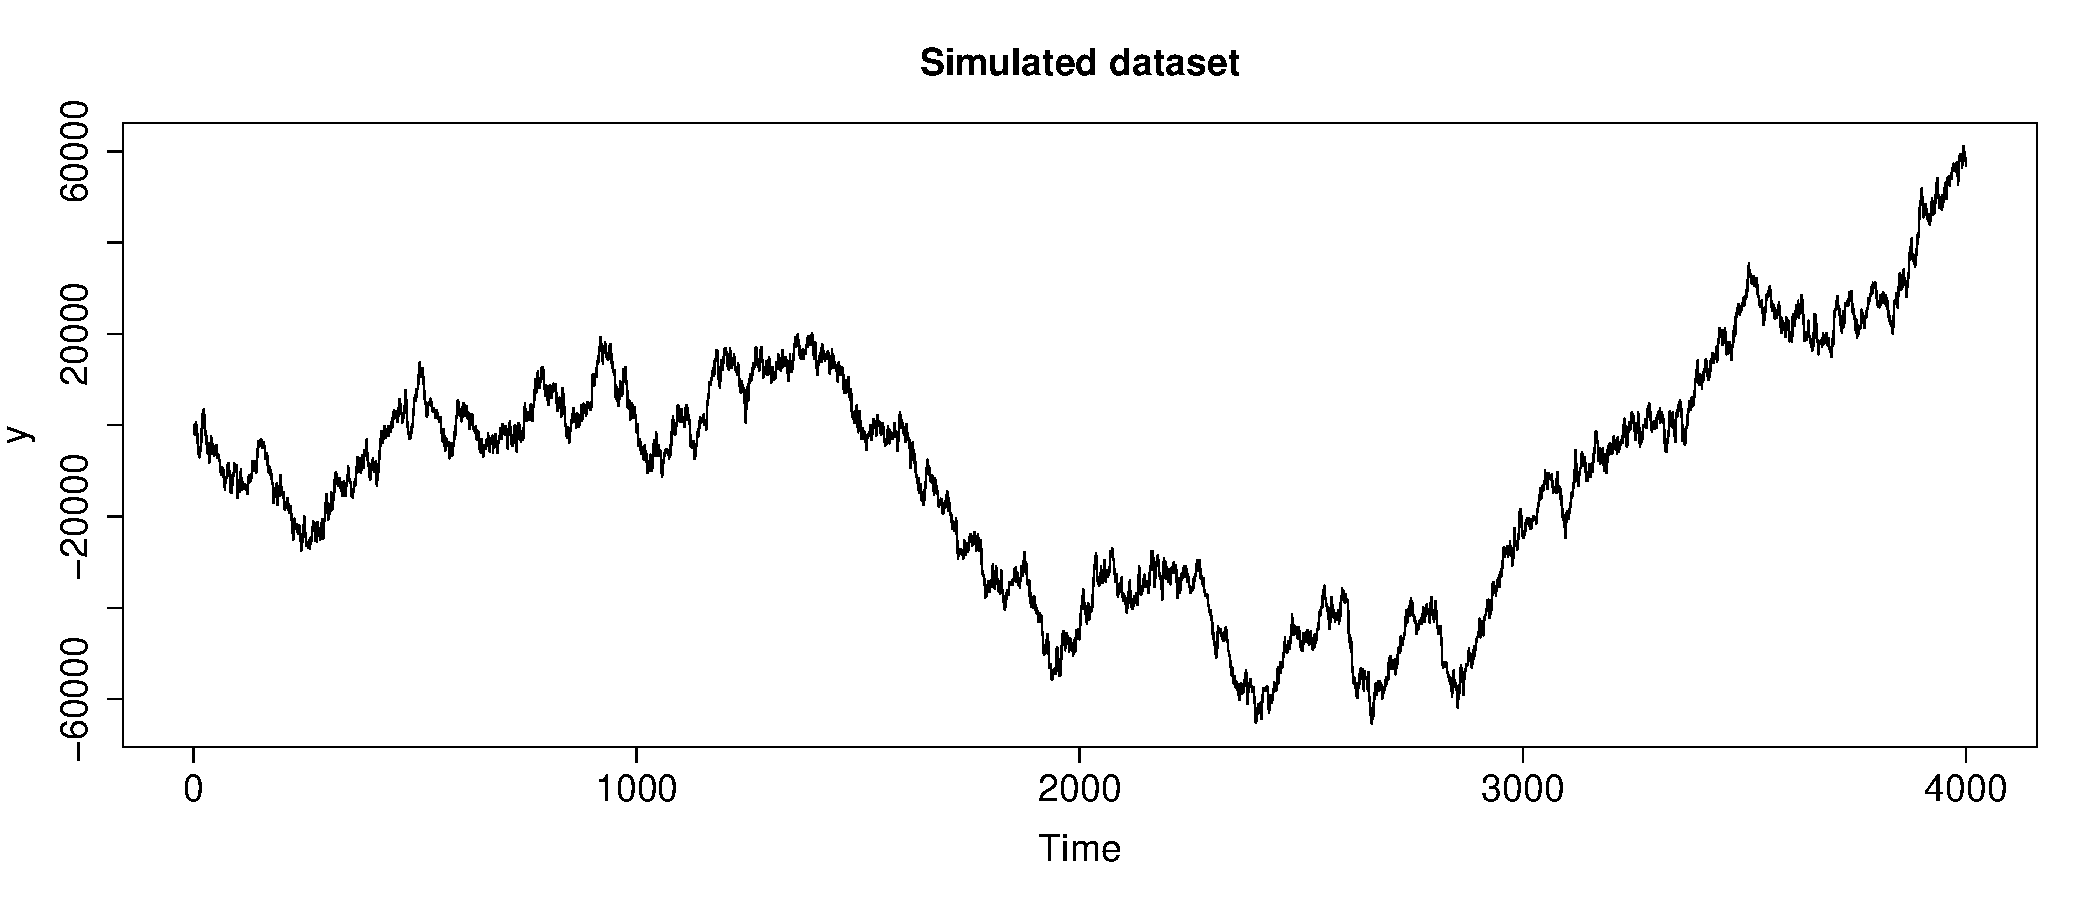
\includegraphics[width=260px]{../plots/arima-sim-1.pdf}}
    \only<2>{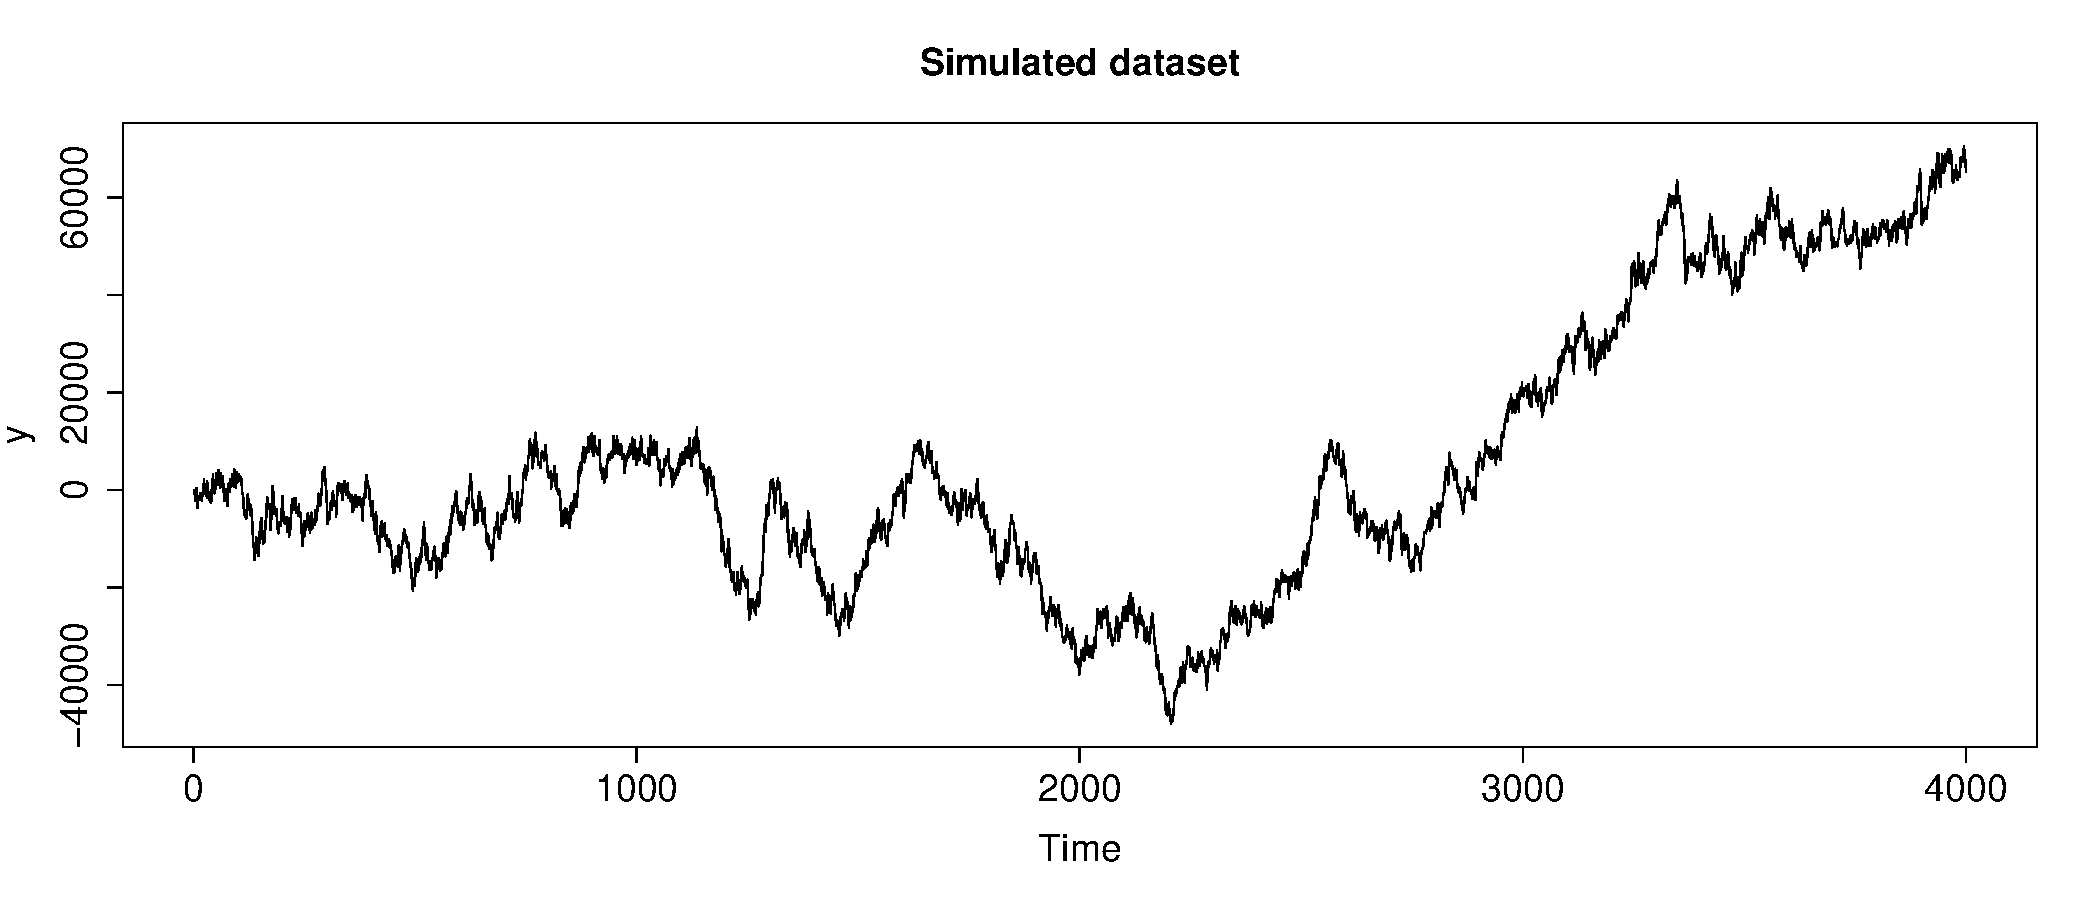
\includegraphics[width=260px]{../plots/arima-sim-2.pdf}}
    \only<3>{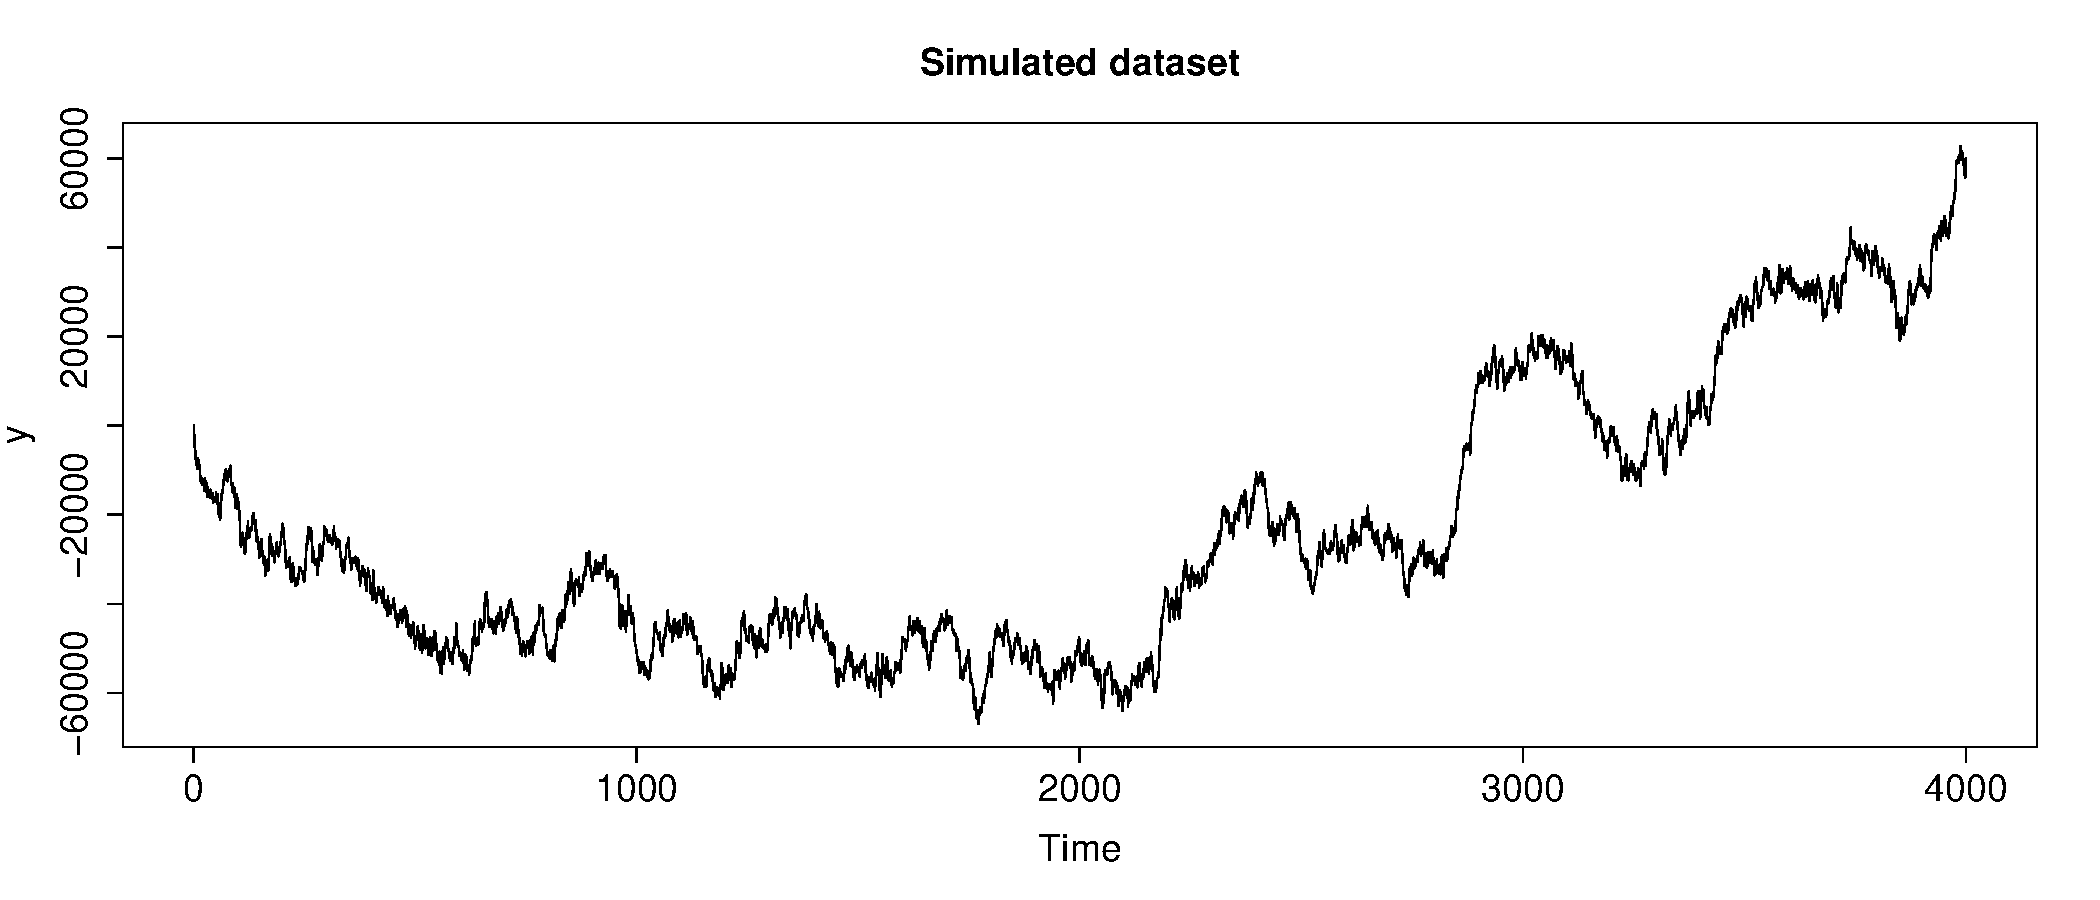
\includegraphics[width=260px]{../plots/arima-sim-3.pdf}}
    \only<4>{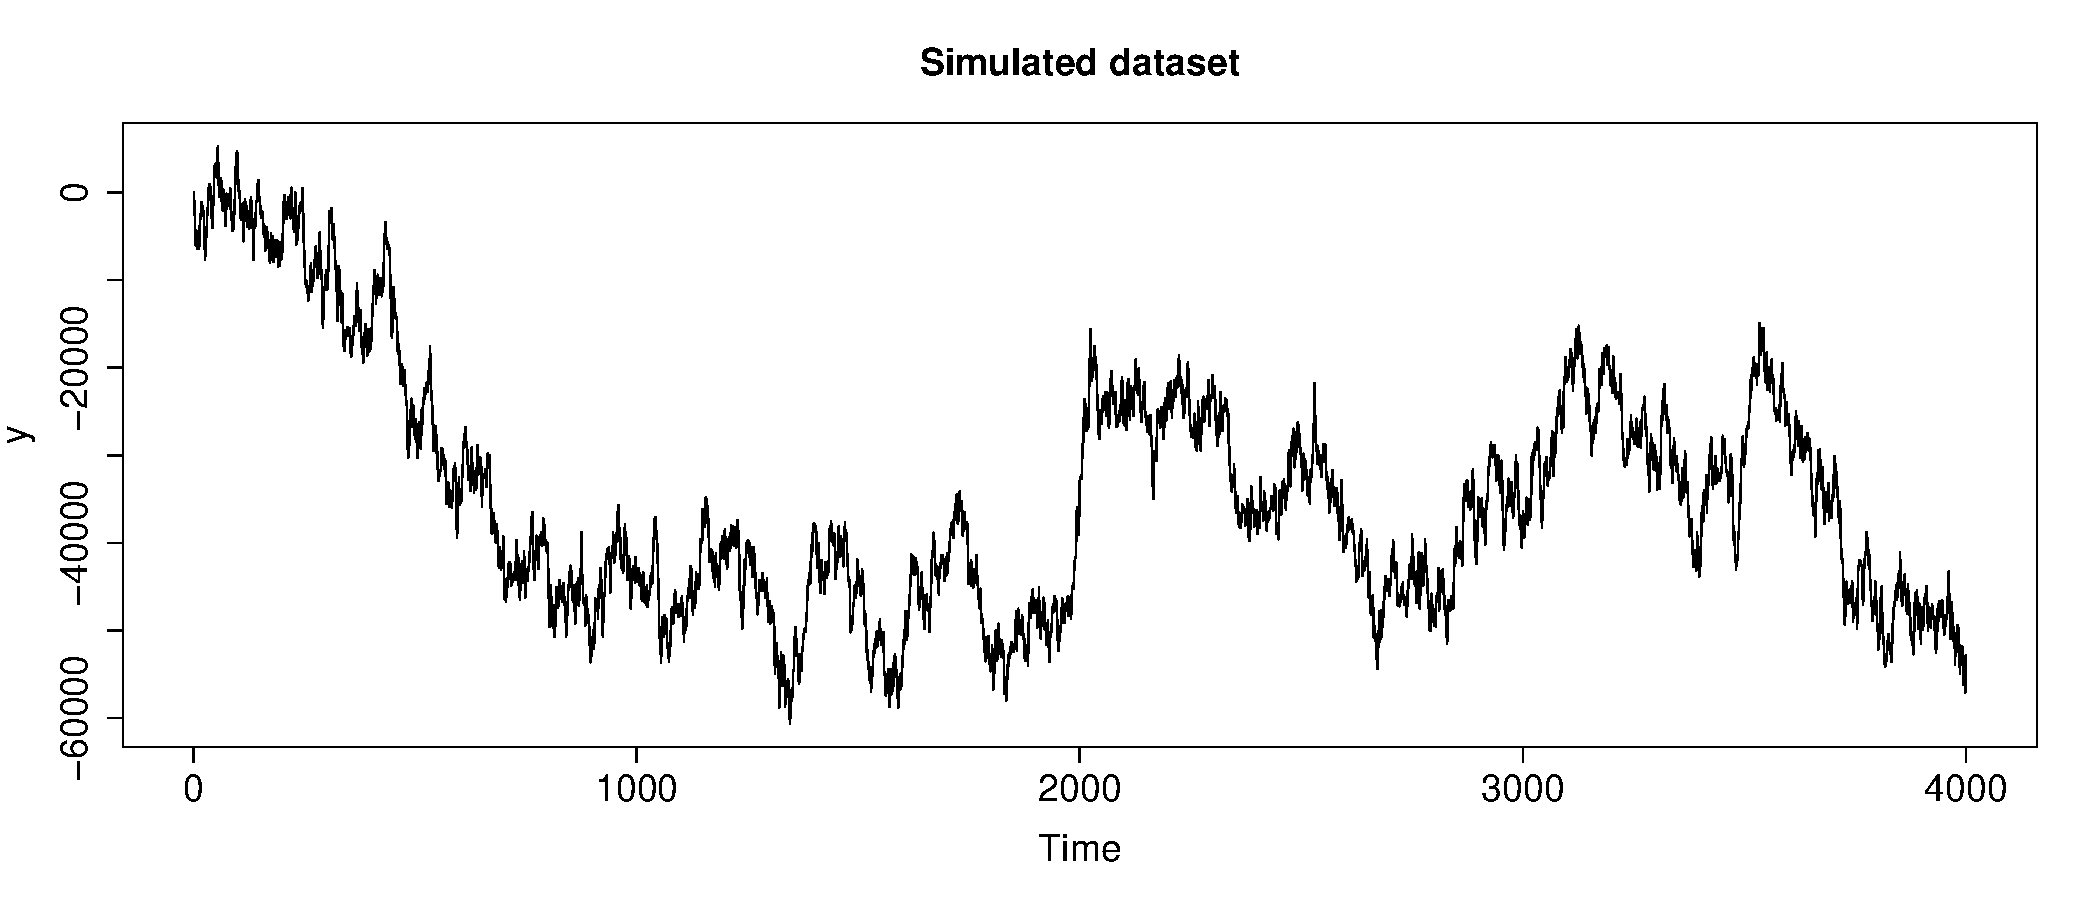
\includegraphics[width=260px]{../plots/arima-sim-4.pdf}}
    \only<5>{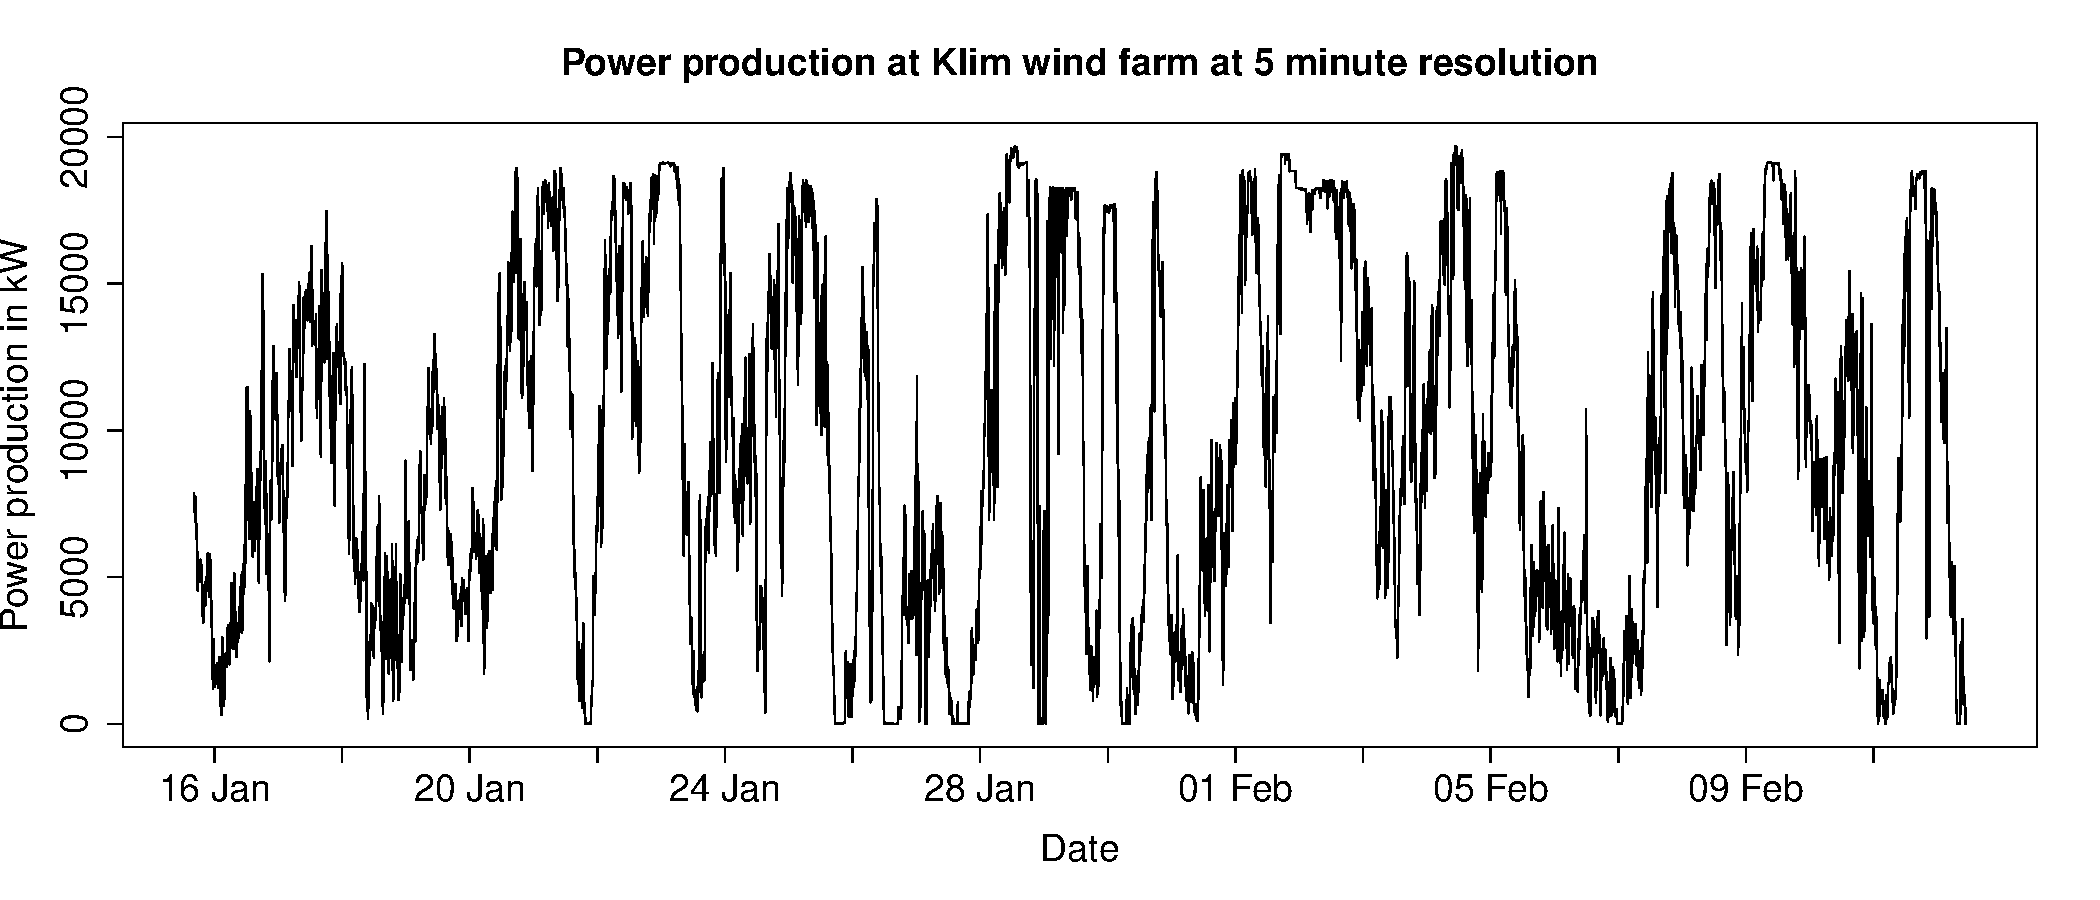
\includegraphics[width=260px]{../plots/training-dataset.pdf}}
    \end{figure}
\end{frame}

\begin{frame}{Hidden Markov Models}
    2-, 3-, and 4-state HMM were fitted to the data. The state dependent distributions as chosen as
    \begin{equation*}
        Y_t\given C_t=i\:\sim\: N(\mu_i, \sigma_i^2)
    \end{equation*}
    
    The best found model was the 4-state model with the state dependent distributions

    \begin{figure}
    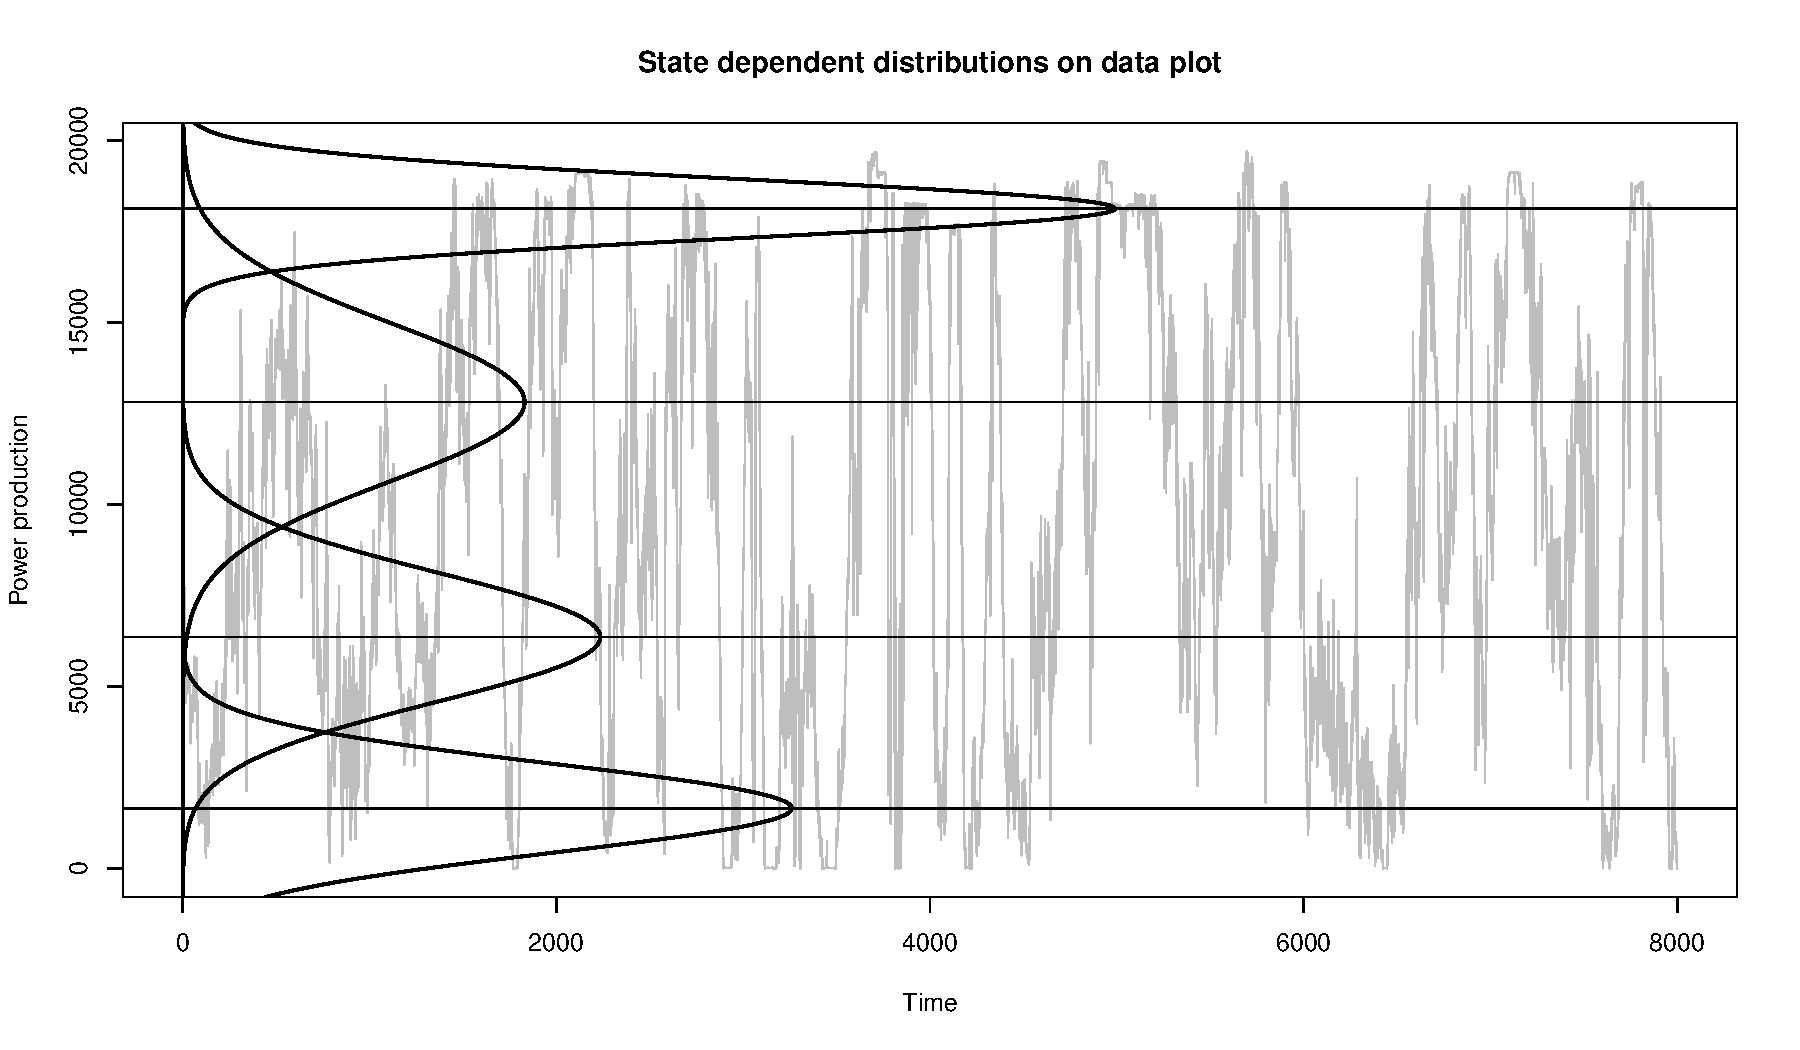
\includegraphics[width=240px]{../plots/4-state-normal-dist-plot.pdf}
    \end{figure}
\end{frame}

\begin{frame}{HMM model check}
    To make an emperical check of the found HMM model, a few datasets were simulated from the found model.
    \begin{figure}
    \only<1>{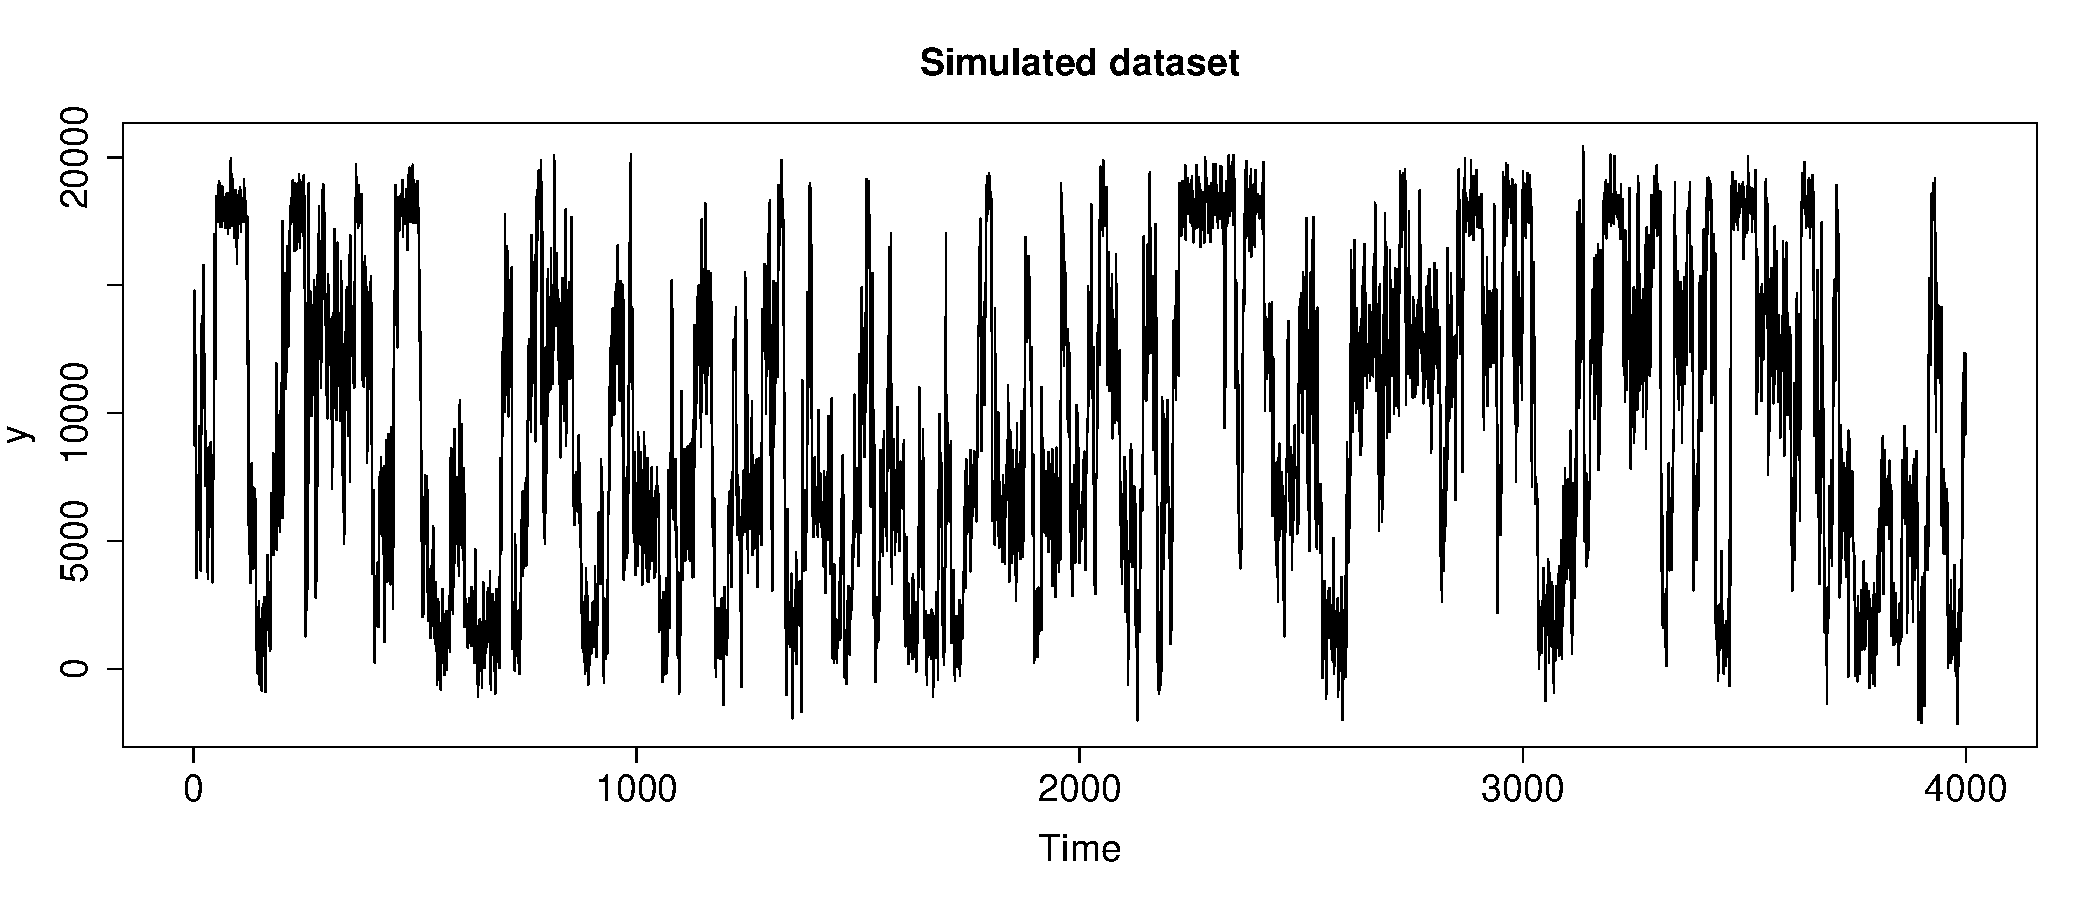
\includegraphics[width=260px]{../plots/4-state-hmm-sim-1.pdf}}
    \only<2>{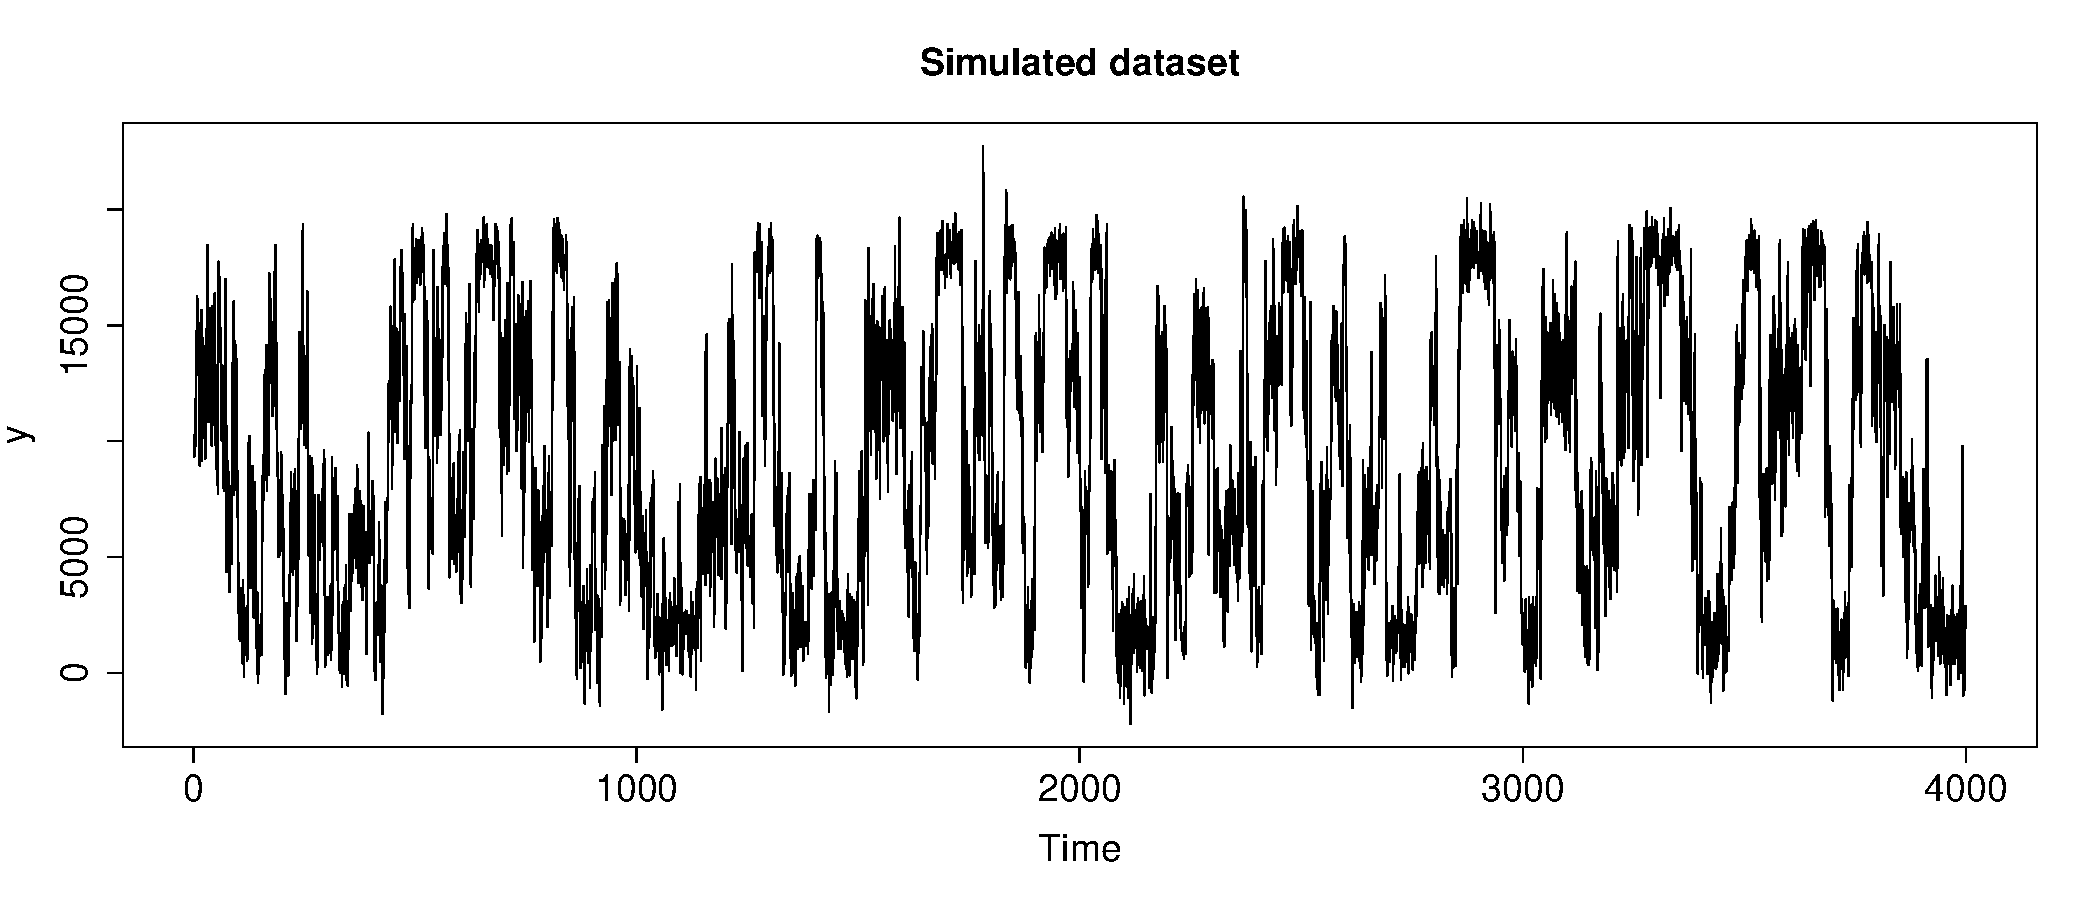
\includegraphics[width=260px]{../plots/4-state-hmm-sim-2.pdf}}
    \only<3>{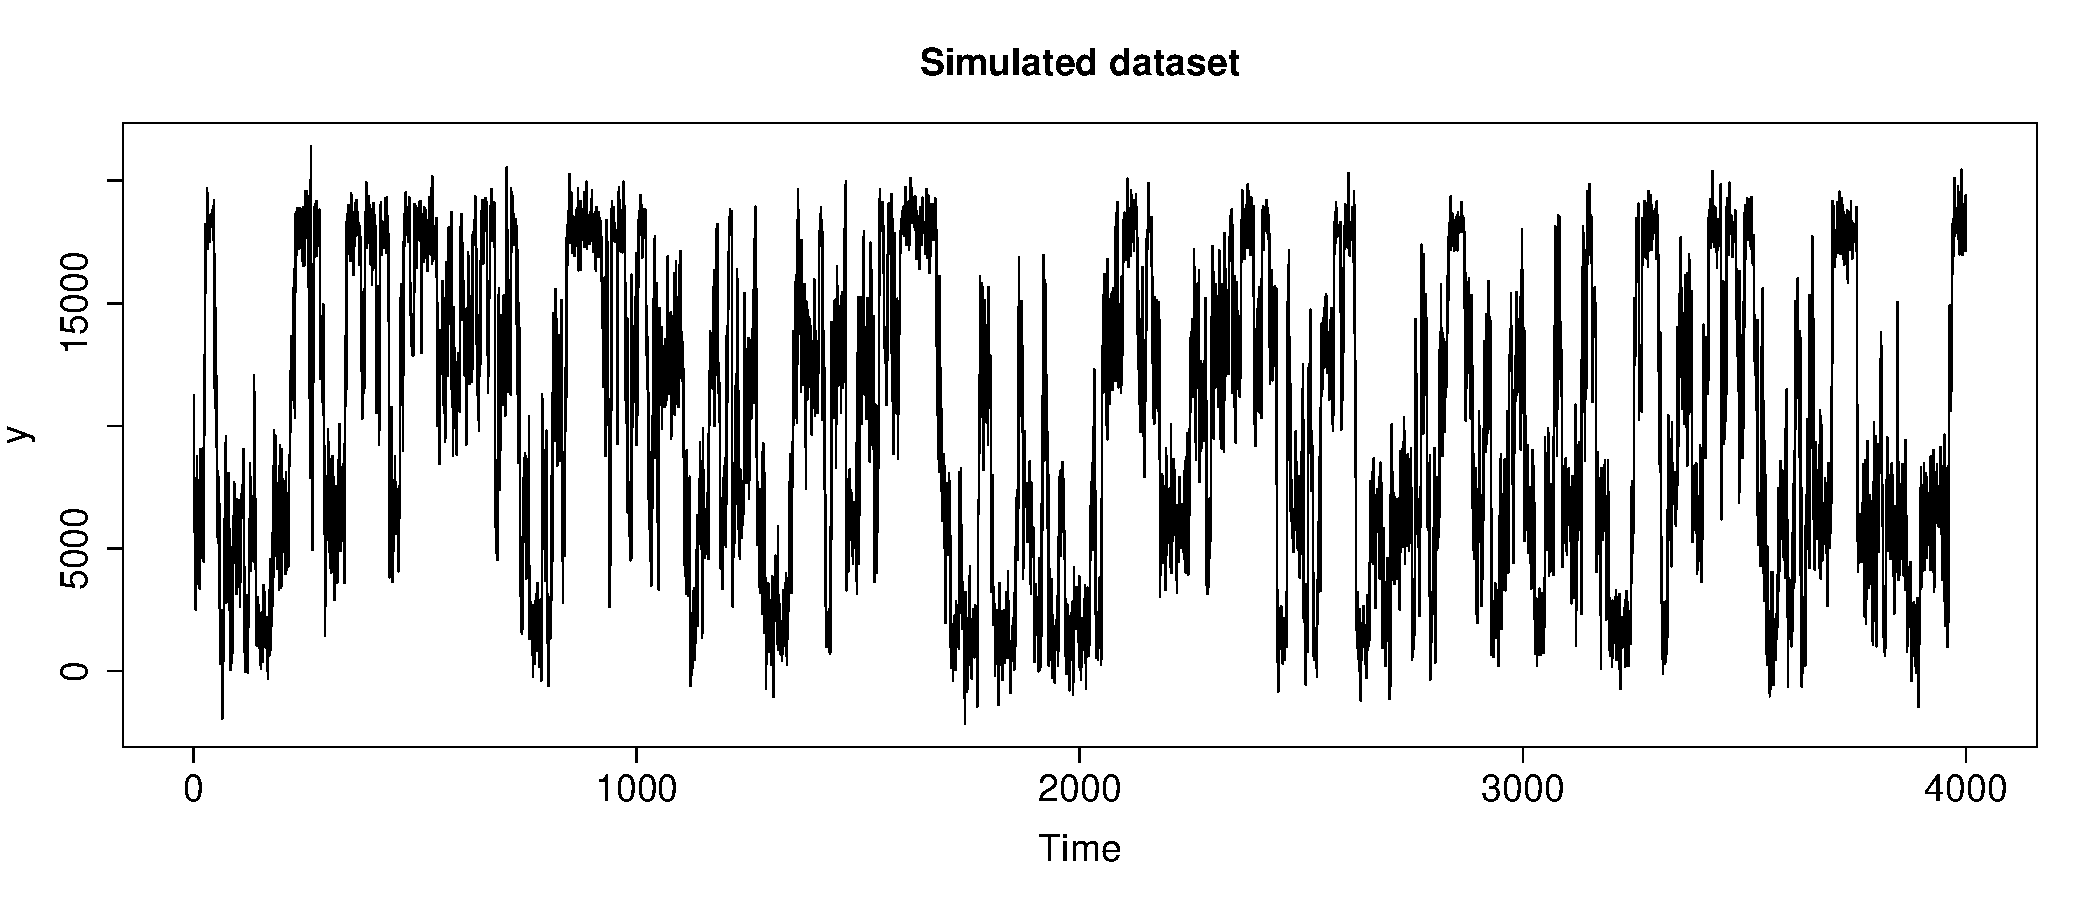
\includegraphics[width=260px]{../plots/4-state-hmm-sim-3.pdf}}
    \only<4>{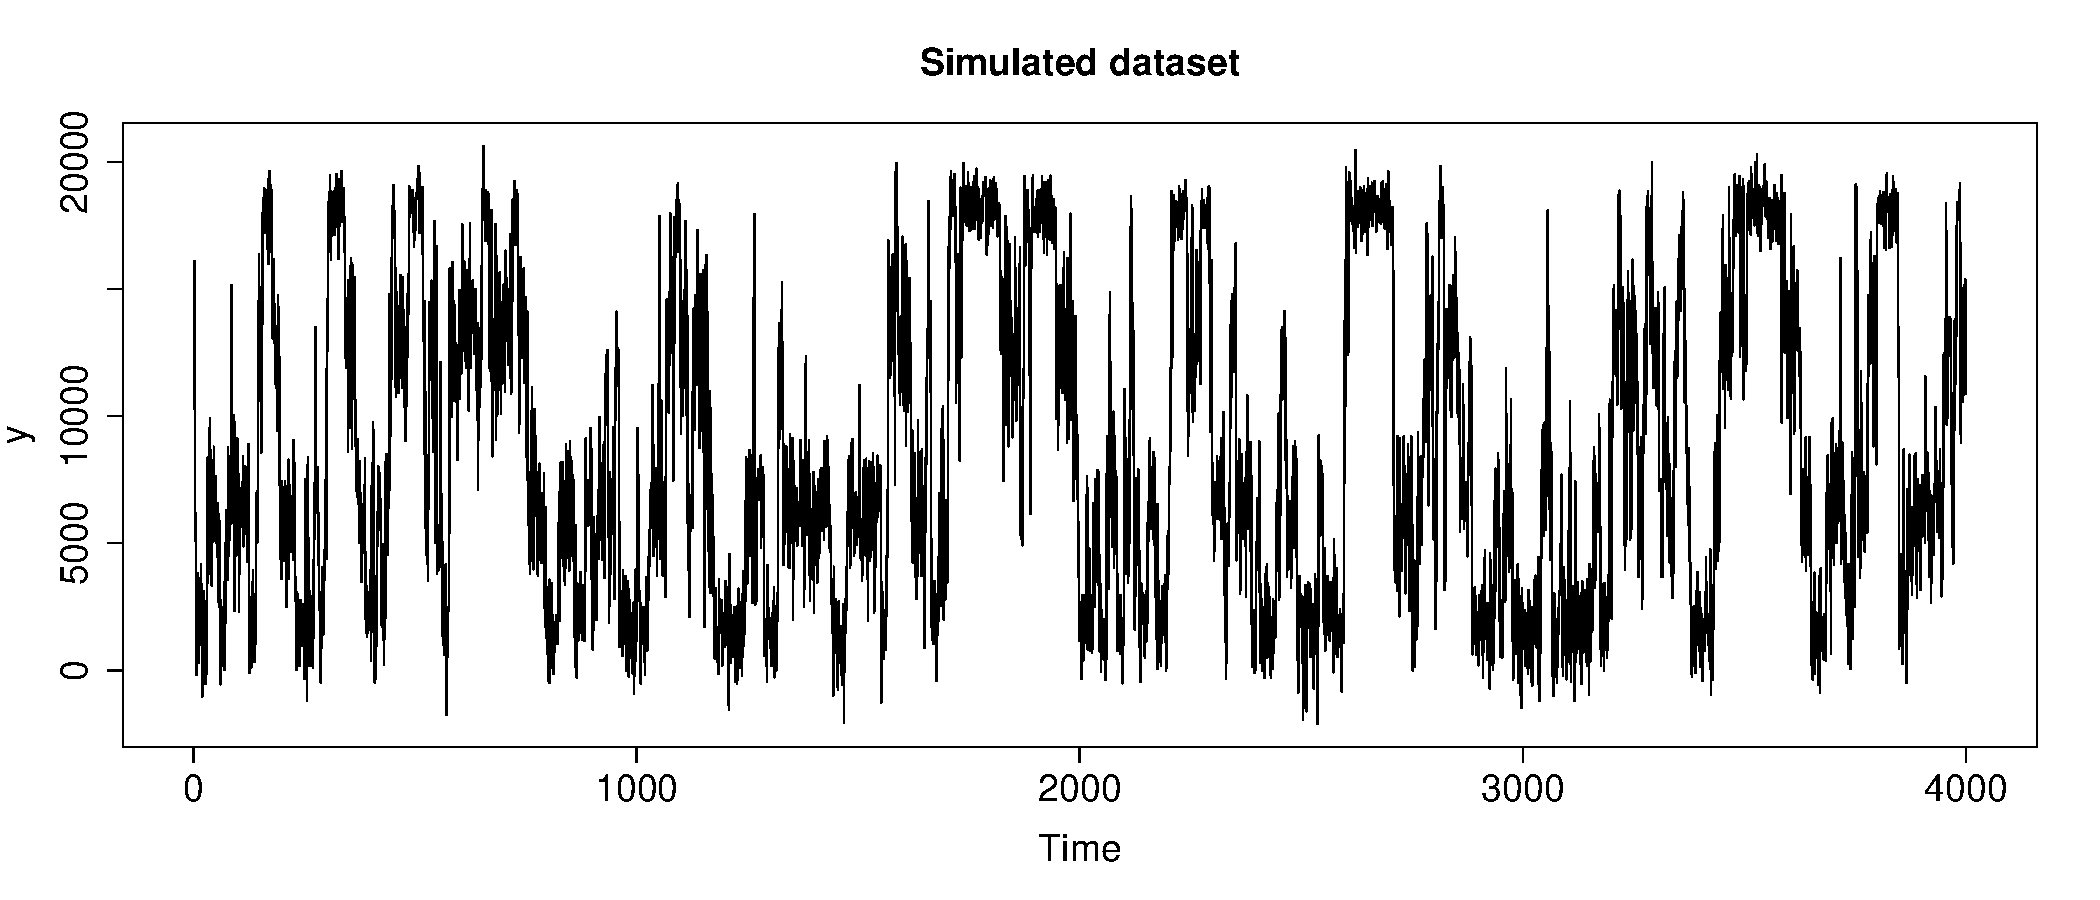
\includegraphics[width=260px]{../plots/4-state-hmm-sim-4.pdf}}
    \only<5>{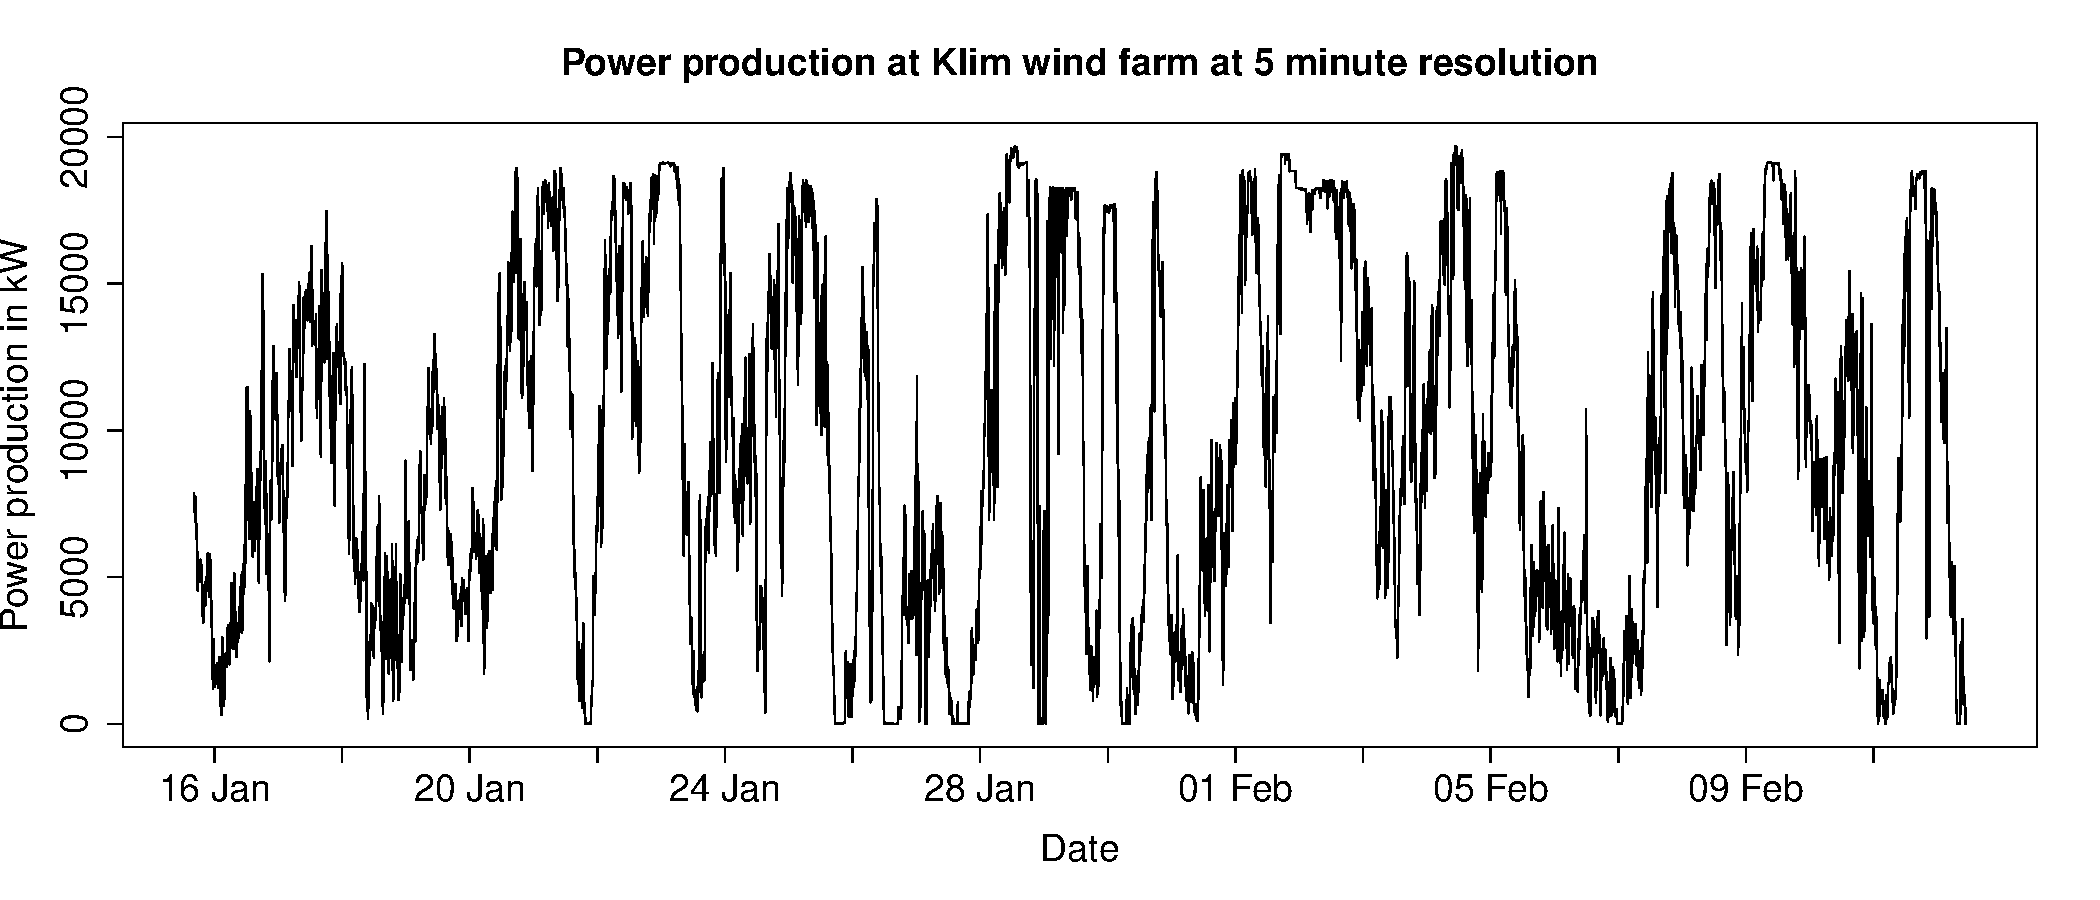
\includegraphics[width=260px]{../plots/training-dataset.pdf}}
    \end{figure}
\end{frame}

\begin{frame}{One-step predictions}
    Had troubles with all one-step prediction distributions being almost identical. Maybe it can be explained by the fact that
    \begin{equation*}
        \textrm{Pr}(Y_{t+1}=y\given\myvec{Y}^{(t)} = \myvec{y}^{(t)}) = \myvec{\phi}_t\myvec{\Gamma}\myvec{P}(y)\myvec{1}^{'}
    \end{equation*}
    where
    \begin{equation*}
        \myvec{\phi}_t = \frac{\myvec{\alpha}_t}{\myvec{\alpha}_t\myvec{1}^{'}}
    \end{equation*}
    If eg. the absolute value of the elements in $\myvec{\alpha}_t$ are of the order $70000$, then differences between elements in $\myvec{\alpha}_t$ and $\myvec{\alpha}_{t+1}$ of the order $100$ will not change $\myvec{\phi}_t$ much.
\end{frame}

\begin{frame}{One-step predictions continued}
    \begin{figure}
    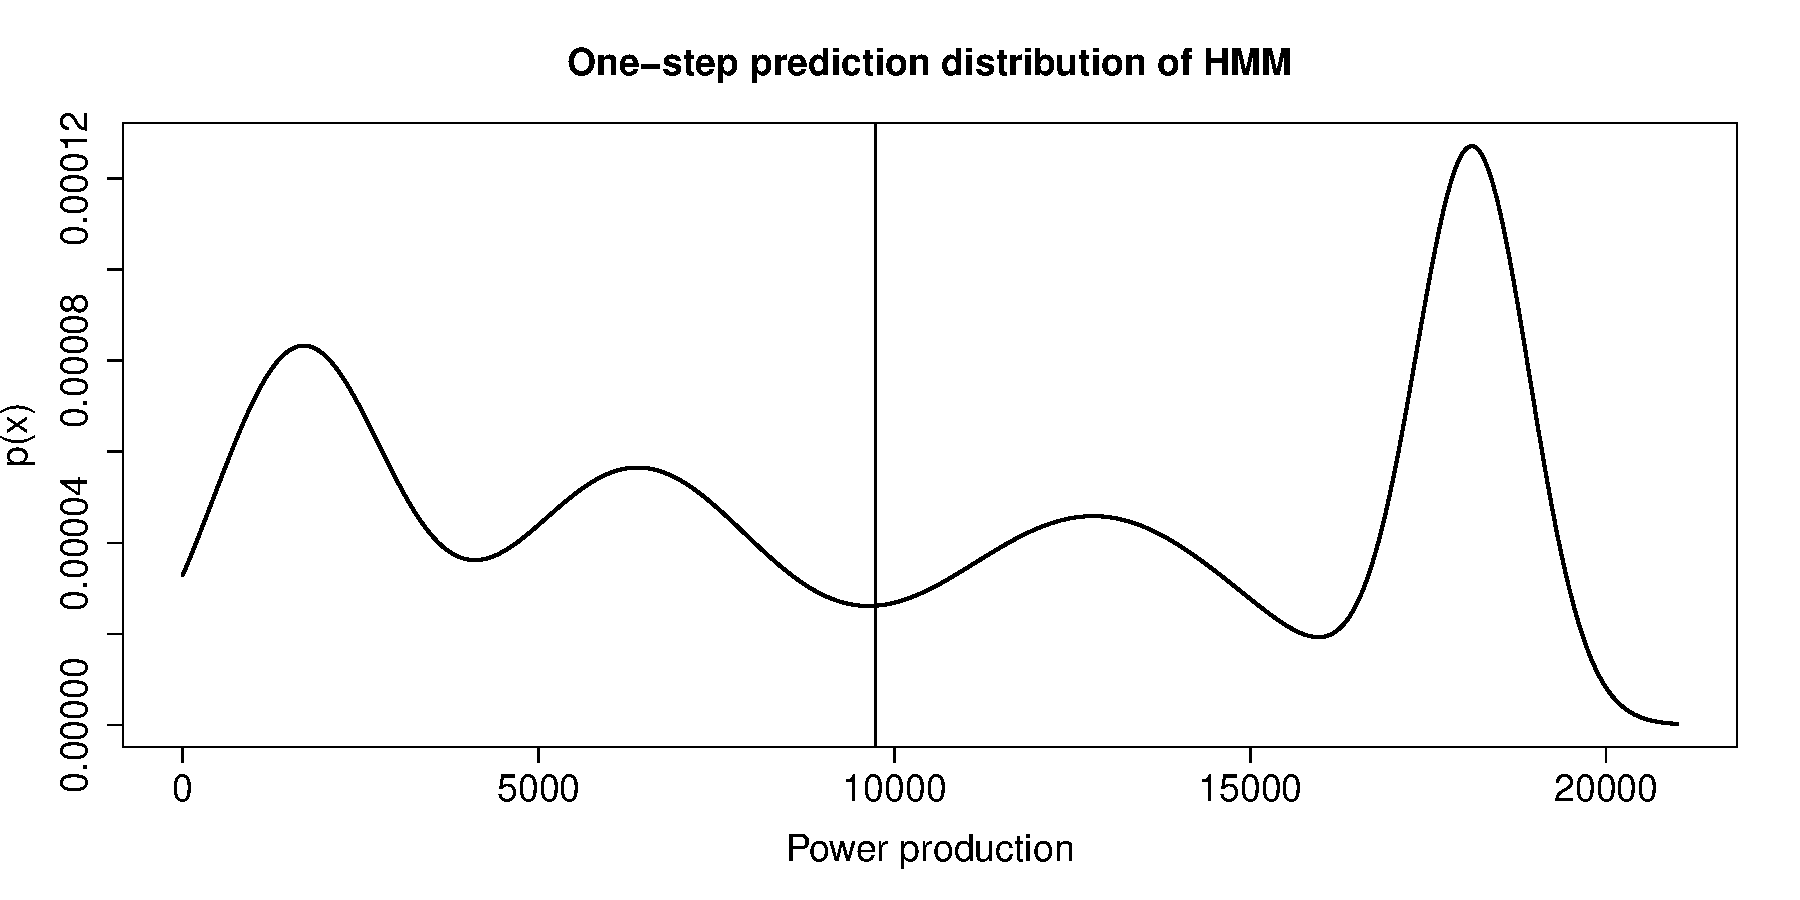
\includegraphics[width=260px]{../plots/one-step-dist.pdf}
    \end{figure}
    Also $\myvec{\phi}_t\approx\myvec{\delta}$, so the prediction distributions was almost the marginal distribution of $Y_t$.
\end{frame}

\begin{frame}{Questions}
    Time for some questions...
\end{frame}


\end{document}
